\documentclass[pscyr]{hedwork}
\usepackage[russian]{babel}
\usepackage{hedmaths}
\usepackage{graphicx}
\graphicspath{{images/}}

\usepackage{color}
\usepackage[colorlinks,linkcolor=black,urlcolor=black]{hyperref}
\renewcommand{\UrlFont}{\rm\small}

\faculty{Факультет электроники и вычислительной техники}
\department{физики}
\subject{дисциплине\\<<Методы и средства физического эксперимента>>}
\topic{Измерение электрического заряда. Типы приборов\\и их конструкция}
\student[f]{студентка группы Ф-469\\Слоква В. И.}
\teacher[m]{старший преподаватель\\Аршинов А. В.}

\begin{document}
  \maketitle
  \tableofcontents

  \section{Приборы, измеряющие заряд}
  \subsection{Электроскоп}
  Чтобы определить наличие у тела электрического заряда, пользуются простым
  прибором, который называется электроскопом. Электроскоп основан на свойстве
  двух предметов, заряженных электричеством одинакового рода, отталкиваться друг
  от друга.

  Этот прибор изображён на рис.~\ref{picElec}. Он состоит из стеклянной банки,
  закрытой пробкой, через которую проходит металлический стержень. На том конце
  стержня, который находится внутри банки, укреплены два тонких продолговатых
  металлических листочка, а на наружном конце находится металлический шарик.
  Если к шарику прикоснуться стеклянной палочкой, заряженной электричеством, то
  это стеклянное электричество перейдёт по стержню на листочки. Оба листочка
  окажутся заряженными электричеством одинакового рода (положительным), и
  поэтому они оттолкнутся друг от друга и примут наклонное положение. Это и
  показано на рис.~\ref{picElec}.

  \begin{figure}[ht]
    \center
    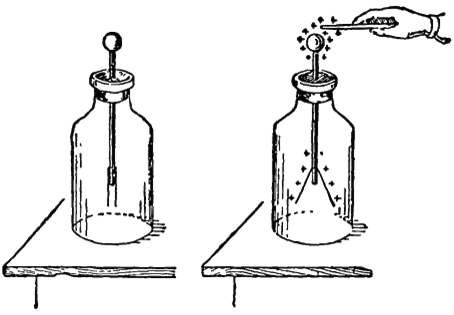
\includegraphics{sl_1_1}
    \parbox{.8\textwidth}{\caption{Листочки электроскопа (справа) раздвинулись,
      что свидетельствует о наличии заряда} \label{picElec}}
  \end{figure}

  Если ещё раз натереть стеклянную палочку и снова прикоснуться ею к шарику, то
  листочки электроскопа разойдутся ещё больше. Это происходит потому, что мы
  зарядили электроскоп дважды или, как говорят, подвели к нему двойное
  количество электричества. Чем больше электричества мы имеем, тем более заметно
  оно себя проявляет.

  \subsection{Механический электрометр}
  В обычных лабораторных опытах для обнаружения и измерения электрических
  зарядов используется электрометр~-- прибор, состоящий из металлического
  стержня и стрелки, которая может вращаться вокруг горизонтальной оси
  (рис.~\ref{picMechElec}). Стержень со стрелкой изолирован от металлического
  корпуса. При соприкосновении заряженного тела со стержнем электрометра,
  электрические заряды одного знака распределяются по стержню и стрелке. Силы
  электрического отталкивания вызывают поворот стрелки на некоторый угол, по
  которому можно судить о заряде, переданном стержню электрометра.

  \begin{figure}[ht]
    \center
    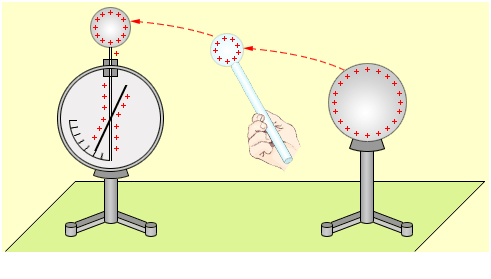
\includegraphics[width=.65\textwidth]{sl_2_1} \hspace{1em}
    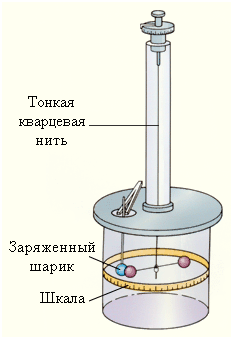
\includegraphics[width=.3\textwidth]{sl_2_2} \\
    \parbox{.65\textwidth}{\caption{Работа с электрометром} \label{picMechElec}}
    \hspace{1em}
    \parbox{.3\textwidth}{\caption{Крутильные весы Кулона} \label{picScales}}
  \end{figure}

  Электрометр является достаточно грубым прибором; он не позволяет исследовать
  силы взаимодействия зарядов. Впервые закон взаимодействия неподвижных зарядов
  был открыт французским физиком Ш.~Кулоном в 1785~г. В своих опытах Кулон
  измерял силы притяжения и отталкивания заряженных шариков с помощью
  сконструированного им прибора~-- крутильных весов (рис.~\ref{picScales}),
  отличавшихся чрезвычайно высокой чувствительностью. Так, например, коромысло
  весов поворачивалось на \( 1^\circ \) под действием силы порядка
  \( 10^{-9} \)~Н.

  Идея измерений основывалась на предположении о том, что если заряженный шарик
  привести в контакт с точно таким же незаряженным, то заряд первого разделится
  между ними поровну. Таким образом, был указан способ изменять заряд шарика в
  два, три и т.~д. раз.

  \subsection{Измерение заряда с помощью баллистического гальванометра}

  Заряд конденсатора измеряют с помощью баллистического гальванометра.

  Баллистический метод является одним из приемов не только электрических, но и
  магнитных измерений. Баллистический гальванометр относится к приборам
  магнито-электрической системы, схематичное устройство которых показано на
  рисунке~\ref{picGalv}.

  \begin{figure}[ht]
    \center
    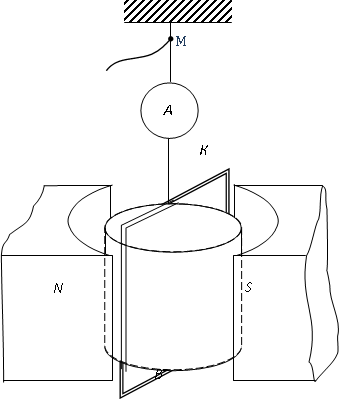
\includegraphics[width=.4\textwidth]{sl_3_1}
    \caption{Устройство приборов магнито-электрической системы}
    \label{picGalv}
  \end{figure}

  Между полюсами постоянного магнита \emph{NS} для создания радиального
  магнитного поля помещен стальной цилиндр \emph{B}. Цилиндр закреплен
  неподвижно. В зазоре между полюсами магнита и цилиндром может свободно
  вращаться рамка \( K \) с обмоткой из тонкой проволоки, подвешенная на
  металлической или кварцевой нити \( M \). Для отсчета углов поворота рамки
  служит зеркальце \( A \), на которое падает световой луч от осветительного
  устройства.

  Баллистический гальванометр служит для измерения заряда, длительность
  \( \tau \) протекания которого по цепи мала по сравнению с периодом \( T \)
  собственных колебаний рамки. Баллистический гальванометр отличается от обычных
  зеркальных гальванометров увеличенным значением момента инерции \( I \) его
  подвижной системы. Если через гальванометр пропустить кратковременный импульс
  тока \( \tau \ll T \), то на рамку в каждый момент времени действует вращающий
  момент, обусловленный взаимодействием тока \( i \) с магнитным полем:
  \( M = i\beta \), где \( \beta \)~-- коэффициент, зависящий от конструктивных
  особенностей прибора; \( i \)~-- мгновенное значение тока. Благодаря большому
  моменту инерции рамка за малое время \( \tau \) практически не успевает выйти
  из положения равновесия, но она приобретает угловую скорость \( \omega_0 \) и,
  следовательно, кинетическую энергию \( I\omega_0^2/2 \). Так как ток к этому
  моменту прекратился, то рамка начинает поворачиваться по инерции с начальной
  скоростью \( \omega_0 \) и закручивает нить. В момент остановки рамки вся
  кинетическая энергия переходит в потенциальную энергию закрученной нити
  \( D\phi^2/2 \), где \( D \)~-- постоянная кручения нити; \( \phi \)~--
  максимальный угол отклонения рамки:
  \begin{equation}
    \frac{I\omega_0^2}{2} = \frac{D\phi^2}{2}, \text{ откуда }
    \phi = \omega_2\sqrt{I/D}.
    \label{eq3-1}
  \end{equation}

  Угловую скорость \( \omega_0 \), приобретенную рамкой к моменту прекращения
  импульса тока, найдем из уравнения движения
  \[
    I\der{\omega}{t} = M; \quad I\der{\omega}{t} = \beta i.
  \]

  Проинтегрируем:
  \begin{equation}
    \int\limits_0^{\omega_0} I\,d\omega = \int\limits_0^\tau \beta i\,dt.
    \text{ Так как } \int\limits_0^\tau i\,dt = q, \text{ то }
    I\omega_0 = \beta q,
    \label{eq3-2}
  \end{equation}
  где \( q \)~-- заряд, прошедший через рамку за время \( \tau \). Решая
  совместно уравнения \eqref{eq3-1} и \eqref{eq3-2}, будем иметь
  \( q = \sqrt{ID}\phi/\beta \). На опыте измеряют отклонение светового
  <<зайчика>> (отброс) не в углах, а в делениях шкалы \( n \). Поскольку
  \( n \) и \( \phi \) пропорциональны друг другу, то окончательно можем
  записать \( q = Bn \), где \( B \)~-- коэффициент пропорциональности, который
  называется баллистической постоянной гальванометра. Баллистическая постоянная
  численно равна величине заряда, вызывающего отклонение <<зайчика>> на одно
  деление шкалы. Любой гальванометр может служить в качестве баллистического,
  если выполнено условие \( \tau \ll T \).

  \subsection{Кулонометры}

  Кулонометрическими называют электрохимические методы анализа, основанные на
  измерении количества электричества, прошедшего через электролитическую ячейку
  при электрохимическом окислении или восстановлении вещества на рабочем
  электроде.

  В основе кулонометрии лежат законы Фарадея для электролиза. Математическое
  выражение объединенного закона Фарадея имеет вид:
  \[
    m = \frac{M}{nF}\cdot Q,
  \]
  где \( m \)~-- масса вещества, окисленного (восстановленного) в процессе
  электролиза; \( M \)~-- молярная масса вещества; \( N \)~-- число электронов,
  участвующих в электродной реакции; \( F \)~-- постоянная Фарадея
  (\( F = 96487 \)~Кл/моль); \( Q \)~-- количество электричества.

  Непременными условиями проведения и прямых и косвенных кулонометрических
  определений являются наличие надежного способа измерения количества
  электричества, способа установления конца электрохимической (в прямой
  кулонометрии) или химической (в косвенной кулонометрии) реакции.

  Единицами количества электричества служат кулон (Кл) и фарадей (Ф). Кулон~--
  это количество электричества, переносимое за 1~с при постоянном токе в 1~А,
  т.~е. \( 1\text{ Кл} = 1 \text{ А}\cdot\text{с} \). Фарадей~-- это количество
  электричества, вызывающее электрохимическое превращение 1~моль эквивалентов
  вещества. Фарадей равен \( 6,\!02\cdot10^{23} \) электронов, или 96487~Кл.

  Различают в зависимости от условий проведения прямую кулонометрию и
  кулонометрическое титрование.

  Прямые кулонометрические определения проводятся при постоянном потенциале.

  Установка для потенциостатических кулонометрических определений состоит из
  рабочего электрода, электрода сравнения и вспомогательного электрода. Рабочим
  электродом кулонометрической ячейки обычно служит платиновая пластина или
  ртуть, хотя иногда используют также золотые, серебряные или графитовые
  электроды. Вспомогательный электрод изготовляется из тех же материалов.
  Электродные пространства рабочего и вспомогательного электродов разделены.
  Контакт между ними осуществляется через пористую перегородку. В качестве
  электрода сравнения обычно выбирают каломельный или хлорсеребряный. Количество
  электричества, израсходованное на протекание электрохимической реакции, может
  быть измерено с помощью интеграторов тока или кулонометров, а также определено
  расчетным методом.

  Для определения количества электричества, прошедшего через электролитическую
  ячейку, используют следующие приемы:
  \begin{enumerate}
    \item С помощью интеграторного тока.
    \item Как площадь кривой <<ток-время>>.
    \item С помощью химического интегратора тока~-- кулонометра.
  \end{enumerate}

  Погрешность измерения количества электричества зависит от точности измерения
  времени, поскольку современные приборы позволяют очень точно измерять даже
  небольшие токи.

  Для измерения количества электричества, выделившегося в процессе
  кулонометрического титрования используют кулонометры.

  Кулонометр~-- это электролитическая ячейка, в которой при замыкании цепи
  со~100\%-ным выходом по току протекает электрохимическая реакция известной
  стехиометрии.

  Кулонометр включают последовательно с кулонометрической ячейкой, поэтому за
  время электролиза через обе ячейки протекает одинаковое количество
  электричества. Если по окончании электролиза измерить массу образовавшегося в
  кулонометре вещества, то по формуле Фарадея можно рассчитать количество
  электричества:
  \[
    Q = \frac{m\cdot n\cdot F}{M}.
  \]

  Существуют гравиметрические, газовые и титрационные кулонометры.

  Гравиметрические кулонометры состоят из платинового анода и катода,
  изготовленного из металла, ионы которого находятся в растворе. Количество
  электричества определяют по увеличению массы катода.

  При использовании титрационных кулонометров количество электричества
  определяют путем титрования продукта электродной реакции.

  При применении газовых кулонометров количество электричества определяют по
  объему газа, выделившегося при электролизе, например, при электролизе воды.

  \subsection{Электронный электроскоп}

  \begin{figure}[ht]
    \center
    
\includegraphics{sl_5_1}
    \caption{Схема электронного электроскопа}
    \label{picElElec}
  \end{figure}

  Предлагаемый электроскоп индицирует знак электрического заряда, и его
  относительную величину. При перемещении источника электрического поля или
  заряженного тела относительно электроскопа, показания прибора изменяются
  обратно пропорционально расстоянию во второй степени.

  Электроскоп представляет собою мост постоянного тока, плечами которого
  являются полевой транзистор \emph{VТ1} и резисторы \emph{R1--R4}. В одну
  диагональ моста включен стрелочный индикатор \emph{PA1} с нулем посередине
  шкалы, в другую~-- источник питания \emph{CB1}. В зависимости от знака заряда
  ток стока транзистора либо уменьшается, либо увеличивается. При этом стрелка
  индикатора отклоняется в соответствующую сторону от среднего положения.
  Переменным резистором \emph{RЗ} стрелку индикатора устанавливают на условный
  нуль перед началом демонстрации. Стрелочный индикатор~-- микроамперметр с
  током полного отклонения стрелки от среднего (нулевого) деления шкалы до
  500~мкА. Вывод затвора транзистора <<висит>> в воздухе внутри корпуса, являясь
  антенной-зондом в исследуемом электрическом поле. При работе с электроскопом
  наэлектризованное тело приближают к затвору, и стрелка индикатора показывает
  относительную величину заряда.

  \section{Методы измерения электрического заряда}
  \subsection{Метод преобразования заряда в напряжение}

  На рисунке~\ref{picQ2U} приведены схемы преобразователей заряда в напряжение.
  Если конденсатор \emph{C} был исходно разряжен, то при поступлении на вход
  усилителя по схеме рис.~\ref{picQ2U}а электрического заряда \( q_\text{вх} \)
  на его выходе получим напряжение (предполагая, что \( K \gg 1 \))
  \[
    U_\text{вых} = -q_\text{вх} / C.
  \]
  Переключатель \emph{S}, установленный
  параллельно конденсатору \emph{C}, предназначен для периодического разряда
  этого конденсатора перед очередным измерением.
  
  Усилитель заряда по схеме~\ref{picQ2U}б позволяет получить большой коэффициент
  усиления без чрезвычайного уменьшения емкости \emph{C}. Для этого усилителя
  при нулевых начальных условиях
  \[
    U_\text{вых} = -\frac{q_\text{вх}}{C}\cdot
      \left( 1 + \frac{R_1}{R_2} \right).
  \]

  \begin{figure}[ht]
    \center
    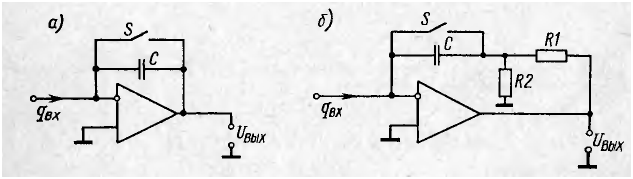
\includegraphics{sl_6_1}
    \caption{Схемы метода преобразования заряда в напряжение}
    \label{picQ2U}
  \end{figure}

  \subsection{Метод магнитной фокусировки}

  Идея метода заключается в следующем. Электронно-лучевая трубка, помещается в
  длинный соленоид, создающий магнитное поле, направленное вдоль оси трубки.
  Электроны вылетают из электронной пушки примерно с одинаковыми продольными
  скоростями. Небольшое напряжение, подаваемое на отклоняющие пластины, изменяет
  только поперечную составляющую скорости. Это означает. Что все электроны в
  магнитном поле будут двигаться по спиралям с одним и тем же шагом \( L \) и,
  следовательно, электроны будут встречаться вновь, пересекая ось пучка на
  расстояниях \( L \), \( 2L \) и т.~д. В этих точках сечение пучка будет
  наименьшим, т.~е. в них электронный пучок будет фокусироваться. Следовательно,
  при изменении магнитного поля изображение пучка на экране будет периодически
  стягиваться в ярко светящееся пятнышко. Если расстояние от пушки до
  экрана~\( l \), то пучок сфокусируется на экране при условии \( l = nL \),
  где \( n = 1, 2, 3, \ldots \), или
  \[
    l = \frac{2\cdot\pi v_\|\cdot n}{e\cdot B_\varphi/m}.
  \]

  Выразив в этой формуле скорость электронов через ускоряющее напряжение,
  получаем выражение для удельного заряда через измеряемые физические величины:
  \[
    \frac{e}{m} = \frac{8\cdot\pi^2\cdot U}{l^2}\cdot
      \left( \frac{n}{B_\varphi} \right)^2.
  \]

  \begin{figure}[ht]
    \center
    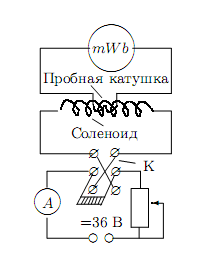
\includegraphics{sl_7_1}
    \caption{Схема измерений по методу магнитной фокусировки}
    \label{picMagFoc}
  \end{figure}

  Основной частью установки является электронно-лучевая трубка, установленная в
  соленоид, создающий магнитное поле. Напряжение на отклоняющие пластины и
  питание проводятся к трубке многожильным кабелем.

  Пучок электронов, вылетающих из катода с разными скоростями (энергия электрона
  \( \sim 0,\!1 \)~эВ), ускоряется анодным напряжением \( \sim 1 \)~кВ.
  Пропустив пучок сквозь две узкие диафрагмы, можно выделить электроны с
  практически одинаковой продольной скоростью \( v_\| \). Небольшое переменное
  напряжение, поступающее на отклоняющие пластины изменяет только поперечную
  составляющую скорости. Угол \( \alpha \) отклонения пучка от оси трубки, таким
  образом, зависит от времени, и электроны <<прочерчивают>> на экране трубки
  светящуюся линию. При увеличении магнитного поля линия на экране сокращается,
  постепенно стягиваясь в точку, а затем снова удлиняется. Второе прохождение
  через фокус происходит в том случае, когда электроны на пути от катода к
  экрану описывают два витка спирали. Третье~-- при трех витках.

  Анодное напряжение, определяющее продольную скорость электронов, измеряется
  электростатическим киловольтметром.

  Магнитное поле в соленоиде создается постоянным током (рис.~\ref{picMagFoc}),
  сила которого регулируется переменным сопротивлением \emph{R} и измеряется
  амперметром \emph{A}. Ключ \emph{K} служит для изменения направления поля в
  соленоиде.

  Величина магнитного поля определяется с помощью измерительной катушки,
  подключенной к милливеберметру. Этот прибор измеряет изменение магнитного
  потока, пронизывающего измерительную катушку, которая намотана на один каркас
  с соленоидом.

  На точность результата может влиять внешнее магнитное поле, особенно
  продольное. Оно не изменяет размеры фокуса, но изменяет величину фокусирующего
  поля. Присутствие внешнего поля можно обнаружить с помощью переполюсовки
  соленоида: при изменении направления поля показания милливеберметра будут
  отличаться, но их полусумма не зависит от наличия постоянного продольного
  поля.

  Определив значение магнитных полей, при которых происходит фокусировка
  электронного пучка, по результатам измерений рассчитывается \( e/m \).

  \subsection{Измерение удельного заряда методом магнетрона}

  Название метода связано с тем, что применяемая в работе конфигурация
  электрического и магнитного полей напоминает конфигурацию полей в
  магнетронах~-- генераторах электромагнитных колебаний сверхвысоких частот.

  \begin{figure}[ht]
    \center
    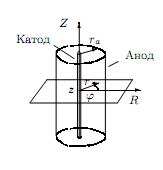
\includegraphics{sl_8_1} \hspace{1em}
    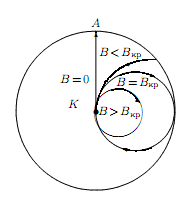
\includegraphics{sl_8_2} \hspace{1em}
    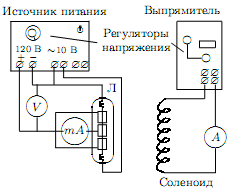
\includegraphics{sl_8_3} \\
    \parbox{10em}{\caption{Схема устройства двухэлектродной лампы}
      \label{picLamp}} \hspace{1ex}
    \parbox{10em}{\caption{Траектории электронов, вылетающих из катода, при
      разных значениях индукции магнитного поля} \label{picElsFly}} \hspace{1ex}
    \parbox{13em}{\caption{Схема измерительной установки} \label{picSchem}}
  \end{figure}

  Движение электронов в этом случае происходит в кольцевом пространстве,
  заключенном между катодом и анодом двухэлектродной электронной лампы
  (рис.~\ref{picLamp}). Нить накала лампы (катод) располагается вдоль оси
  цилиндрического анода, так что электрическое поле между катодом и анодом имеет
  радиальное направление. Лампа помещается внутри соленоида, создающего
  магнитное поле, параллельное оси лампы.

  Рассмотрим траектории электронов. Пусть задан потенциал анода \( U_a \). В
  отсутствие магнитного поля (рис.~\ref{picElsFly}) электрон движется
  прямолинейно по радиусу. При слабом поле траектории несколько искривляются, но
  электроны все же попадают на анод. При некотором критическом значении индукции
  магнитного поля \( B_\text{кр} \) траектории искривляются на столько, что
  только касаются анода. При \( B > B_\text{кр} \) электроны вовсе не попадают
  на анод и возвращаются к катоду. Величину \( B_\text{кр} \) можно найти по
  формуле
  \[
    eU = \frac{m}{2}\left[ \dot{r}^2 + \left( \frac{reB}{2m} \right)^2 \right],
  \]
  при этом радиальная скорость электрона (при радиусе анода) обращается в нуль:
  \[
    U_a = \frac{e B_\text{кр}^2 r_a}{8m}.
  \]

  Отсюда \( e/m \):
  \[
    e/m = \frac{8U_a}{B_\text{кр}^2 r_a}.
  \]

  Последняя формула позволяет вычислить \( e/m \), если при заданном \( U_a \)
  найдено такое значение магнитного поля (или наоборот), при котором электроны
  перестают попадать на анод.

  На рисунке~\ref{picSchem} приведена схема установки для измерения удельного
  заряда. Двухэлектродная лампа \emph{Л} с цилиндрическим анодом специально
  изготовлена из немагнитных материалов. Анод лампы состоит из трех
  металлических цилиндров одинакового диаметра. Два крайних цилиндра
  электрически изолированы от среднего небольшими зазорами и используются при
  измерениях. В качестве катода используется тонкая (диаметром 50~мкм) хорошо
  натянутая вольфрамовая проволока, расположенная по оси всех трех цилиндров
  анодной системы. Катод лампы разогревается переменным током, отбираемым от
  стабилизированного источника питания. С этого источника на анод лампы подается
  постоянное напряжение (0-120~В), регулируемое с помощью потенциометра и
  измеряемое вольтметром \emph{V}.

  Лампа закреплена в соленоиде. Ток, проходящий через соленоид, подается с
  выпрямителя и измеряется амперметром \emph{А}. Индукция магнитного поля в
  соленоиде рассчитывается по току, протекающему через обмотку соленоида.

  Для определения удельного заряда данным методом исследуется зависимость
  анодного тока от тока, протекающего через соленоид, при различных напряжениях
  на аноде лампы. Определив для каждого значения \( U_a \) критическое значение
  индукции магнитного поля, необходимо построить зависимость \( B_\text{кр}^2 \)
  от \( U_a \). По угловому коэффициенту полученной прямой определяется удельный
  заряд электрона \( e/m \).

  \pagebreak
  \renewcommand{\bibname}{Список литературы}

  \begin{thebibliography}{9} \addcontentsline{toc}{section}{Список литературы}
    \bibitem{1} Спектор,~С.~А. Электрические измерения физических величин:
      Методы измерений: Учеб. пособие для вузов~/ С.~А.~Спектор~--
      Л.:~Энергоатомиздат. Ленингр.~отд-ние, 1987.~-- 320~с.
    \bibitem{2} Носители электрического тока в вакууме, металлах и
      полупроводниках: Лабораторные работы №№~4.3, 4.4, 35, 4.11А, 4.11Б,
      4.12~-- М.: Изд-во МФТИ, 2007.~-- 55~с.
    \bibitem{3} Кулонометрические методы анализа. Режим доступа:\\
      \url{http://pharmax.ru/articles/Kulonometricheskie-metody-%
      analiza-article3151.html}\\
      (дата обращения 10.11.2013).
  \end{thebibliography}
\end{document}
